% Template for ICASSP-2016 paper; to be used with:
%          spconf.sty  - ICASSP/ICIP LaTeX style file, and
%          IEEEbib.bst - IEEE bibliography style file.
% --------------------------------------------------------------------------
\documentclass[tikz, multi,dvipsnames,svgnames,x11names]{article}
\usepackage{spconf,amsmath,graphicx,float, amssymb, listings, mathtools, bm}
\usepackage{algorithm}
\usepackage[noend]{algpseudocode}
\usepackage{pifont}
\usepackage[edges]{forest}

\makeatletter
\def\BState{\State\hskip-\ALG@thistlm}
\makeatother

% Example definitions.
% --------------------
\def\x{{\mathbf x}}
\def\L{{\cal L}}

% Title.
% ------
\title{Comparison of Unsupervised Pre-training Methods}
% ---------------
\name{Jifu Zhao}
\address{University of Illinois at Urbana-Champaign\\
		 Department of Nuclear, Plasma, and Radiological Engineering\\
		 Urbana, Illinois 61801, USA}

\begin{document}
\maketitle

% ---------------------------------------------------------------------------------------
\begin{abstract}
Unsupervised per-training methods are very important steps for many applications. In this work, we focused on pre-training feature extraction methods. More specifically, we focus on Principal Component Analysis (PCA), kernel PCA and auto-encoders. By comparing their effect for a multiclass digits classification problem, we give an direct comparison of the performance of different methods.
\end{abstract}

% ---------------------------------------------------------------------------------------
\begin{keywords}
PCA, kernel PCA, Auto-encoder
%PCA, kernel PCA, Auto-encoder
\end{keywords}

% ---------------------------------------------------------------------------------------
\section{Introduction}
\label{sec:intro}

As one important part of artificial intelligence (AI), machine learning has been widely used in our daily lives, such as natural language processing (NLP), zip code recognition, self-driving cars and so on. Among those applications, supervised learning is the most common and perhaps the most powerful form of machine learning \cite{lecun2015deep}. For supervised learning, the choice of appropriate representations of original features is very important \cite{bengio2012deep}. For a long time, most machine learning applications require us to specify the input $\bm{x}$ and target $\bm{y}$. The choice of feature representation $\bm{x}$ is usually determined by experts. And sometimes the input $\bm{x}$ may be just the raw feature without pre-processing. 

Researchers have been working on discovering the hidden structures of the data for years. In this process, several methods have been developed and found to be useful in some domains, such as PCA, Independent Component Analysis (ICA), Non-negative Matrix Factorization (NMF), restricted Boltzmann machine (RBM), Auto-encoders and so on. These methods works in an unsupervised way and the output from these methods are thought to be a transformation of the raw input features. For further learning, some supervised learning mechanisms will be built based on the output from these pre-training methods rather than the raw features. As expected, a good representation can help the supervised learning algorithms work better.

As one of the most widely used methods, PCA is a powerful technique for extracting hidden structures from possibly high-dimension data sets \cite{scholkopf1998nonlinear}. PCA is essentially an eigendecomposition problem \cite{friedman2001elements}. As an orthogonal transformation, however, PCA doesn't work well when the latent variables of the data are non-linearly related to the original data. To extract information in a non-linearly way, many methods has been proposed, such as kernel PCA and auto-encoders.

Kernel PCA was proposed by Sch\"{o}lkopf {\em et~al.}\cite{scholkopf1998nonlinear}. In their work, starting from the traditional PCA algorithm, they found that, after mapping the data from original feature space $\bm{x}$ into a new feature space through some nonlinear function $\bm{\phi(\bm{x})}$, PCA algorithm requires huge amount of computations when the dimensionality of the new feature space is extremely high. Instead of solving this problem explicitly in the new feature space, they extracted the principal components through the so-called kernel matrix. In this way, this problem can be transformed into solving the eigendecomposition problem of the kernel matrix, whose dimensionality is determined by the size of the data set rather than the new feature space. This method is very useful when the new feature space is extremely high (for example, $10^{10}$). Using this method, the authors chose the US Postal Service database for a multicalss classification problem. With only a subset of $3000$ training examples and a soft margin hyperplane classifier, they got a very good accuracy, which was compatible with support vector machine and convolutional neural networks \cite{scholkopf1998nonlinear}.

In addition to kernel PCA, auto-encoder is another commonly used non-linear feature extraction method. Auto-encoders use the input as the target, trying to find a reconstruction $\bm{r(\bm{x})} = \bm{g(h(\bm{x}))}$ through encoder $\bm h(\cdot)$ and decoder $\bm g(\cdot)$ \cite{bengio2012deep}. In most cases, an auto-encoder system is a multi-layer deep neural network which has a bottleneck structure. Auto-encoders can be trained through back-propagation. However, it works well only if we have a good initialization, especially when there are many hidden layers. To get a good initialization, Hinton and Salakhutdinov \cite{hinton2006reducing} then proposed an effective way which utilize a stack of RBMs for pre-training. They first built a stack of RBMs, each having only one layer of feature detectors. The learned feature representations from one RBM were used as the input to the next RBM. Since each RBM was trained separately, it was much easier than training a deep auto-encoder. After pre-training, the learned weights of the RBMs were used as the initialization for the corresponding deep auto-encoders. The auto-encoder was then trained further through back-propagation. Following the above steps, they applied this method on several data sets, including MNIST data set \cite{lecun1998gradient}, Olivetti face data set \cite{samaria1994parameterisation} and Reuters Corpora \cite{lewis2004rcv1}, which showed good results.

In this work, we focus on the comparison of several unsupervised per-training methods. More specifically, we focus on PCA, kernel PCA and auto-encoders (with and without RBM initialization). In section \ref{sec:method}, we gave some brief review for PCA, kernel PCA and auto-encoders. In section \ref{sec:experiment}, we conducted experiments on MNIST data set using PCA kernel PCA and auto-encoder. Finally, in section \ref{sec:conclusion}, we gave some conclusions and potential future works.

% ---------------------------------------------------------------------------------------
\section{Methods}
\label{sec:method}

% ---------------------------------------------------------------------------------------
\subsection{PCA}
\label{pca}

The goal of PCA is to find a lower-dimension space such that the variance of the orthogonal projection of the original data is maximized \cite{bishop2007pattern}. PCA is essentially performed by solving the eigendecomposition problem of the covariance matrix. The PCA algorithm can be summarized in Algorithm \ref{PCA_algo}.

\begin{algorithm}[htb]
\caption{PCA in Feature Space}
\label{PCA_algo}
\begin{algorithmic}[1]
\Procedure{PCA}{\it X}
	\State $\text{given input:} \  X_{n \times m} \leftarrow \begin{bmatrix} \bm{x}_1; \bm{x}_2; \cdots; \bm{x}_n \end{bmatrix}^T$
	\State $\text{de-mean: } \  x_{ij} \leftarrow x_{ij} - \bar{x}_j \  or \  x_{ij} \leftarrow \frac{x_{ij} - \bar{x}_j}{s_j}$
	\State $\text{covariance matrix:} \  C \leftarrow \frac{1}{n} X^T X$
	\State $\text{eigendecomposition:} \  \lambda \bm{u} = C \bm{u}$
	\State $\text{first k eigenvectors:} \  U_{m \times k} \leftarrow \begin{bmatrix} \bm{u}_1; \bm{u}_2; \cdots; \bm{u}_k \end{bmatrix}$
	\State $\text{project the test data} \  \bm{x}: \  \bm{p} \leftarrow U^T \bm{x}$
\BState \bf finish
\EndProcedure
\end{algorithmic}
\end{algorithm}

% ---------------------------------------------------------------------------------------
\subsection{Kernel PCA}
\label{kernelPCA}

Suppose that we first map the input $\bm{x}$ from original feature space $\mathbb{R}^m$ into a new feature space $\mathbb{F}^d$ through some function $\bm{\phi(\bm{x})}$ (usually $d > m$ or even $d \gg m$):
\begin{equation}
\label{eq1}
\bm{\phi}: \mathbb{R}^m \rightarrow \mathbb{F}^d
\end{equation}

For simplicity, let's first suppose that the projected data is centered, that is $\sum_{i=1}^n \bm{\phi}(\bm{x}_i)=\bm 0$. Then the covariance matrix in this space is:
\begin{equation}
\label{eq2}
C = \frac{1}{n} \sum_{i=1}^n \bm{\phi}(\bm{x}_i) \bm{\phi}(\bm{x}_i)^T
\end{equation}
and its eigendecomposition can be written as:
\begin{equation}
\label{eq3}
C\bm{v} = \lambda \bm{v}
\end{equation}

Note that $\bm v$ can be written as a linear combination of $\bm{\phi}(\bm{x}_i)$:
\begin{equation}
\label{eq4}
\bm{v} = \sum_{i=1}^n \alpha_i \bm{\phi}(\bm{x}_i)
\end{equation}
From equation (\ref{eq2}), (\ref{eq3}) and (\ref{eq4}) 
\begin{equation}
\label{eq5}
\frac{1}{n} \sum_{i=1}^n \bm{\phi}(\bm{x}_i) \bm{\phi}(\bm{x}_i)^T  \sum_{j=1}^n \alpha_j \bm{\phi}(\bm{x}_j) = \lambda \sum_{i=1}^n \alpha_i \bm{\phi}(\bm{x}_i)
\end{equation}

Now, if we multiply both sides of equation (\ref{eq5}) by $\bm{\phi}(\bm{x}_k)^T$ and express $\bm{\phi}(\bm{x}_i)^T \bm{\phi}(\bm{x}_j)$ as $k(\bm{x}_i, \bm{x}_j)$, we can get:
\begin{equation}
\label{eq6}
\frac{1}{n} \sum_{i=1}^n k(\bm{x}_k, \bm{x}_i) \sum_{j=1}^n \alpha_j k(\bm{x}_i, \bm{x}_j) = \lambda \sum_{i=1}^n \alpha_i k(\bm{x}_k, \bm{x}_i)
\end{equation}
Now, let's define $n \times n$ kernel matrix $K$ to be:
\begin{equation}
\label{eq7}
K_{ij} = k(\bm{x}_i, \bm{x}_i) = \bm{\phi}(\bm{x}_i)^T \bm{\phi}(\bm{x}_j)
\end{equation}	
In matrix form, this is:
\begin{equation}
\label{eq8}
K^2 \bm{\alpha} = n\lambda K \bm{\alpha}
\end{equation}
where $\bm{\alpha}$ is a n-dimensional column vector. We can find $\bm{\alpha}_i$ and $\lambda_i$ by solving the following eigendecomposition problem:
\begin{equation}
\label{eq9}
K \bm{\alpha}_i = n\lambda_i \bm{\alpha}_i
\end{equation}

Also, note that we require $\bm{v}_i^T \bm{v}_i = 1$, so we need to normalize $\bm{\alpha}_i$ such that:
\begin{equation}
\label{eq10}
\lambda_i n \bm{\alpha}_i^T \bm{\alpha}_i = 1
\end{equation}

From above equations, the projection of any given data $\bm{x}$ onto the ith eigenvector $\bm{v}v_i$ can be written as:
\begin{equation}
\label{eq11}
p_i(\bm x) = \bm{\phi(x)}^T \bm{v}_i = \sum_{j=1}^n \alpha_{ij} k(\bm{x}, \bm{x}_j)
\end{equation}

At the begining, we assume that the projected data is centered. However, there is no guarantee that the projected data set given by $\phi(\bm{x}_n)$ has zero mean, so we need manually centralize the projected data \cite{bishop2007pattern} by:
\begin{equation}
\label{eq12}
K' = K - \mathbb{I}_nK/n - K\mathbb{I}_n/n + \mathbb{I}_nK\mathbb{I}_n/n^2
\end{equation}
where $\mathbb{I}_n$ stands for $n \times n$ matrix with all values equal to $1$.

The above kernel PCA algorithm can be summarized in Algorithm \ref{kernelPCA_algo}.

\begin{algorithm}[htb]
\caption{Kernel PCA}
\label{kernelPCA_algo}
\begin{algorithmic}[1]
\Procedure{kernel PCA}{\it X}
	\State $\text{given input:} \  X_{n \times m} \leftarrow \begin{bmatrix} \bm{x}_1; \bm{x}_2; \cdots; \bm{x}_n \end{bmatrix}^T$
	\State $\text{kernel matrix} \  K_{n \times n}: \  k_{ij} \leftarrow k(\bm{x}_i, \bm{x}_j)$
	\State $K' \leftarrow K - \mathbb{I}_nK/n - K\mathbb{I}_n/n + \mathbb{I}_nK\mathbb{I}_n/n^2$
	\State $\text{eigendecomposition:} \ \bm{\alpha}_1, \bm{\alpha}_2, \cdots \leftarrow n \lambda \bm{\alpha} = K' \bm{\alpha}$
	\State $\text{normalization:} \  \bm{\alpha}_i \leftarrow n \lambda_i \bm{\alpha}_i^T \bm{\alpha}_i = 1$
	\State $\text{project the test data} \  \bm{x}$
%	\State $\text{project the test data} \  \bm{x}:  \  p_i(\bm{x}) \leftarrow \sum_{j=1}^n \alpha_{ij} k(\bm{x}, \bm{x}_j)$
\BState \bf finish
\EndProcedure
\end{algorithmic}
\end{algorithm}

Some commonly used kernels includes:
\begin{equation}
\label{eq13}
\textit{Polynomial kernel:} \ \  k(\bm{x}, \bm{y}) = (\gamma \bm{x}^T \bm{y} + c)^d
\end{equation}
\begin{equation}
\label{eq14}
\textit{Gaussian kernel:} \ \  k(\bm{x}, \bm{y}) = exp(-\gamma ||\bm{x} - \bm{y}||^2)
\end{equation}

% ---------------------------------------------------------------------------------------
\subsection{Auto-encoders}
\label{autoencoder}

As mentioned in section \ref{sec:intro}, auto-encoders use the input as the target, trying to reconstruct the input through encoder and decoder \cite{bengio2012deep}. A simple $5$ layer auto-encoder system is shown in Figure \ref{fig:autoencoder}.
\begin{figure}[htb]
\centering
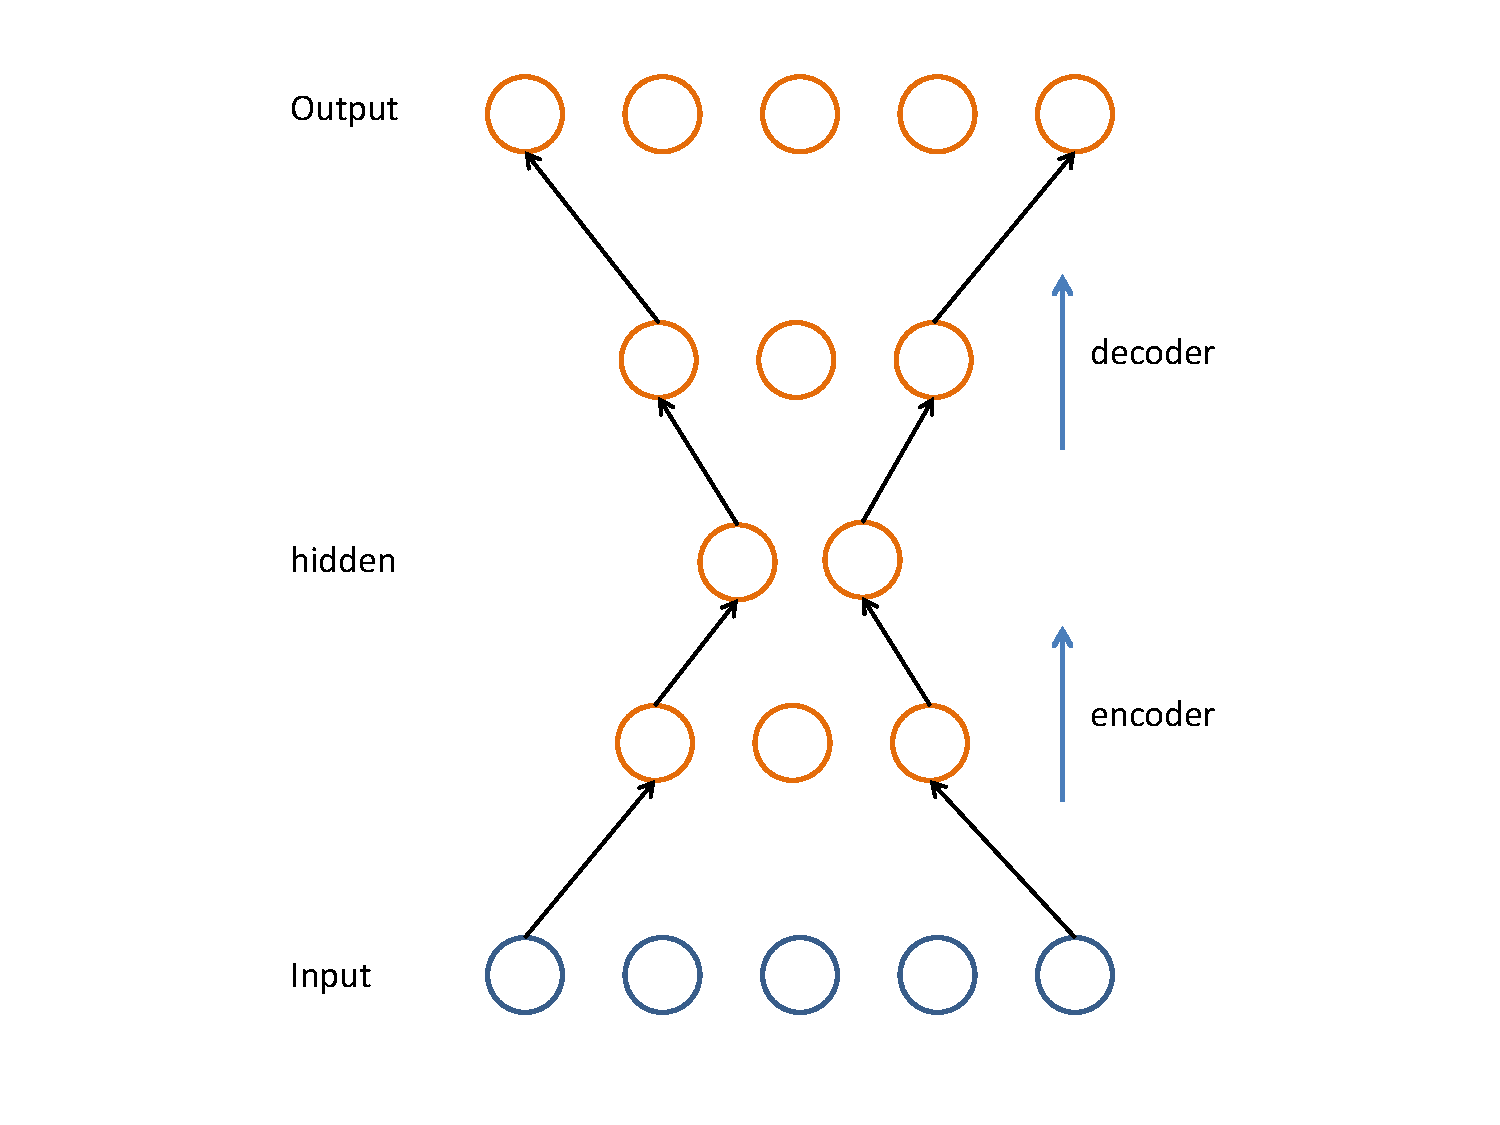
\includegraphics[width=8cm]{./figures/autoencoder.pdf}
\caption{Illustration of auto-encoder system.}
\label{fig:autoencoder}
\end{figure}

Suppose the auto-encoder has $L$ layers, where $1_{st}$ layer is the input $\bm x$ and $L_{th}$ layer is the output layer. In this work, we use sigmoid function as the activation function:
\begin{equation}
sigmoid(z) = \frac{1}{1 + exp(-z)}
\end{equation}
For the output layer, we use the squared-error as the cost function:
\begin{equation}
E = \frac{1}{2}\sum_{i=1}^n \sum_{j=0}^m (y_{ij}^{(L)} - x_{ij})^2
\end{equation}
Followed the back-propagation rule, the update rule can be easily derived.


% ---------------------------------------------------------------------------------------
\section{Experiments}
\label{sec:experiment}

\subsection{Data}
\label{data}
In this work, we used the MNIST dataset \cite{lecun1998gradient} to compare the performance of different pre-training methods. The MNIST data set contains a huge amount of handwirtten digits, including $55000$ training examples, $5000$ validation examples and $10000$ test examples. There are $10$ classes which correspond to digits from $0$ to $9$. Each example is a $28 \times 28$ pixel grayscale image and the pixel values range from $0$ to $1$.

Since the main goal of this work was to compare different pre-training methods, in this work, we only implemented a simple 10-way multiclass logistic regression neural network for final classification.

\subsection{PCA vs. kernel PCA}
\label{pca-kpca}

In this part, we focus on the comparison of PCA and kernel PCA. More specifically, we apply PCA and kernel PCA model with different polynomial kernels (as denoted in equation \ref{eq13}). Due to huge computation requirement for kernel PCA, we select a subset of $20,000$ training examples to build the kernel PCA model, then transform training and test data according to this model. After choosing different number of transformed features, we perform multiclass classification. The test accuracy are shown in Table \ref{table:test_acc}.

%\begin{table*}[htb]
%	\centering
%	\caption{Training Accuracy for Different Kernels}
%	\label{table:train_acc}	
%	\begin{tabular}{c c c c c c c c c c c}
%		\hline \hline
%			   & \multicolumn{10}{c}{Polynomial Kernel Degrees} \\
%		\cline{2-11}
%    Components & 1 	 	& 2 	 &	3 	   & 4 		& 5 	 & 6 	  & 7 	   & 8 	    & 9 	 & 10 \\[0.1cm]
%		\hline
%		32	   & 0.8934 & 0.8685 &	0.8734 & 0.8775 & 0.8800 & 0.8819 & 0.8832 & 0.8847 & 0.8862 & 0.8869\\[0.1cm]
%		64	   & 0.9113 & 0.8852 &	0.8910 & 0.8951 & 0.8974 & 0.9007 & 0.9026 & 0.9050 & 0.9068 & 0.9086\\[0.1cm]
%		128	   & 0.9216 & 0.8919 &	0.9002 & 0.9063 & 0.9113 & 0.9162 & 0.9208 & 0.9245 & 0.9274 & 0.9301\\[0.1cm]
%		256    & 0.9286 & 0.9006 &	0.9146 & 0.9244 & 0.9311 & 0.9363 & 0.9396 & 0.9430 & 0.9460 & 0.9483\\[0.1cm]
%		512	   & 0.9347 & 0.9168 &	0.9297 & 0.9386 & 0.9445 & 0.9493 & 0.9535 & 0.9561 & 0.9593 & 0.9612\\[0.1cm]
%		784	   & 0.9356 & 0.9241 &	0.9374 & 0.9463 & 0.9522 & 0.9566 & 0.9602 & 0.9629 & 0.9654 & 0.9673\\[0.1cm]
%		1024   & N.A.	& 0.9257 &	0.9404 & 0.9492 & 0.9555 & 0.9600 & 0.9638 & 0.9667 & 0.9691 & 0.9708\\[0.1cm]
%		2048   & N.A.	& 0.9289 &	0.9453 & 0.9543 & 0.9615 & 0.9668 & 0.9704 & 0.9735 & 0.9763 & 0.9787\\[0.1cm]
%		4096   & N.A.	& 0.9289 &	0.9482 & 0.9565 & 0.9658 & 0.9713 & 0.9747 & 0.9786 & 0.9818 & 0.9837\\[0.1cm]
%		8192   & N.A.	& 0.9302 &	0.9503 & 0.9570 & 0.9690 & 0.9748 & 0.9772 & 0.9817 & 0.9852 & 0.9881\\[0.1cm]
%		16384  & N.A.	& 0.9315 &	0.9521 & 0.9592 & 0.9717 & 0.9783 & 0.9801 & 0.9847 & 0.9889 & 0.9915\\[0.1cm]
%		\hline	
%	\end{tabular}
%\end{table*}

\begin{table*}[htb]
	\centering
	\caption{Test Accuracy for Kernel PCA}
	\label{table:test_acc}	
	\begin{tabular}{c c c c c c c c c c c}
		\hline \hline
			   & \multicolumn{10}{c}{Polynomial Kernel Degrees} \\
		\cline{2-11}
    Components & 1 	 	& 2 	 &	3 	   & 4 		& 5 	 & 6 	  & 7 	   & 8 	    & 9 	 & 10 \\[0.1cm]
		\hline
		32	   & 0.9005 & 0.8777 &	0.8816 & 0.8846 & 0.8877 & 0.8901 & 0.8912 & 0.8932 & 0.8938 & 0.8944\\[0.1cm]
		64	   & 0.9155 & 0.8952 &	0.8992 & 0.9013 & 0.9044 & 0.9075 & 0.9088 & 0.9115 & 0.9130 & 0.9146\\[0.1cm]
		128	   & 0.9222 & 0.8984 &	0.9062 & 0.9122 & 0.9161 & 0.9197 & 0.9239 & 0.9273 & 0.9302 & 0.9329\\[0.1cm]
		256    & 0.9235 & 0.9058 &	0.9153 & 0.9255 & 0.9320 & 0.9365 & 0.9404 & 0.9437 & 0.9462 & 0.9488\\[0.1cm]
		512	   & 0.9255 & 0.9220 &	0.9316 & 0.9391 & 0.9445 & 0.9483 & 0.9520 & 0.9557 & 0.9584 & 0.9597\\[0.1cm]
		784	   & 0.9242 & 0.9262 &	0.9385 & 0.9451 & 0.9498 & 0.9536 & 0.9578 & 0.9602 & 0.9626 & 0.9641\\[0.1cm]
		1024   & N.A.	& 0.9276 &	0.8403 & 0.9475 & 0.9530 & 0.9569 & 0.9604 & 0.9632 & 0.9656 & 0.9672\\[0.1cm]
		2048   & N.A.	& 0.9291 &	0.9436 & 0.9510 & 0.9587 & 0.9629 & 0.9662 & 0.9690 & 0.9702 & 0.9716\\[0.1cm]
		4096   & N.A.	& 0.9293 &	0.9454 & 0.9525 & 0.9610 & 0.9652 & 0.9676 & 0.9712 & 0.9728 & 0.9753\\[0.1cm]
		8192   & N.A.	& 0.9305 &	0.9466 & 0.9514 & 0.9630 & 0.9672 & 0.9693 & 0.9722 & 0.9739 & 0.9763\\[0.1cm]
		16384  & N.A.	& 0.9314 &	0.9473 & 0.9534 & 0.9635 & 0.9683 & 0.9709 & 0.9730 & 0.9746 & 0.9769\\[0.1cm]
		\hline	
	\end{tabular}
\end{table*}

With polynomial kernels, we have more features to be chosen. As a result, the test accuracy gets improved a lot, which is shown clearly in Table \ref{table:test_acc}. Our best result is with $10$-degree polynomial kernel and $16384$ features. The training accuracy and test accuracy are $0.9915$ and $0.9769$ respectively (as a comparison, the training accuracy and test accuracy is only $0.9340$ and $0.9267$ when classified using the original $784$ features as the input).

% ---------------------------------------------------------------------------------------
\subsection{PCA vs. Auto-encoder}
\label{pca-autoencoder}

In this part, we focus on bottleneck auto-encoders. More specifically, we focused on the $5$-layer structure which is shown in Figure \ref{fig:autoencoder}.

Each MNIST example has $784$ features. Choosing $784$ features as the input, we can build the auto-encoder with different number of hidden nodes, for example, $784$-$512$-$256$-$512$-$784$, where the decoded feature representation has $256$ dimensions. Then, the decoded feature representations are used as the input into a multiclass classification neural network as described in Section \ref{data} and \ref{pca-kpca}. The test accuracy is shown in Table \ref{table:test_acc_auto}. The number of first hidden layer nodes are shown in horizontal direction while the number of second hidden layer nodes are shown in vertical direction. For comparison purpose, the results from PCA are also shown in Table \ref{table:test_acc_auto}.

%\begin{table}[htb]
%	\centering
%	\caption{Training Accuracy for Auto-encoder and PCA}
%	\label{table:train_acc_auto}	
%	\begin{tabular}{c c c c c }
%		\hline \hline
%			   & \multicolumn{3}{c}{Auto-encoder (1st layer)} & \\
%		\cline{2-4}
%    2nd layer   &	128    & 256 	& 512	 & PCA	 \\[0.1cm]
%		\hline
%		16      &	0.7591 & 0.8184 & 0.8453 & 0.8511 \\[0.1cm]
%		32	    &	0.8119 & 0.8621 & 0.8710 & 0.8934 \\[0.1cm]
%		64	    &	0.8627 & 0.8901 & 0.8925 & 0.9113 \\[0.1cm]
%		128	    &	0.8949 & 0.9041 & 0.9149 & 0.9216 \\[0.1cm]
%		256     &	N.A.   & 0.9325 & 0.9392 & 0.9286 \\[0.1cm]
%		\hline	
%	\end{tabular}
%\end{table}

\begin{table*}[htb]
	\centering
	\caption{Test Accuracy for Auto-encoder and PCA}
	\label{table:test_acc_auto}	
	\begin{tabular}{c c c c c c c c c}
		\hline \hline
		 & \multicolumn{3}{c}{Without RBMs (1st layer)} &  & \multicolumn{3}{c}{With RBMs (1st layer)}\\
		\cline{2-4} \cline{6-8}
    2nd layer  &	128    & 256 	& 512    & PCA 	  & 128    & 256 	& 512    \\[0.1cm]
		\hline
		16     &	0.7698 & 0.8339 & 0.8524 & 0.8551 & 0.8550 & 0.8687 & 0.8742 \\[0.1cm]
		32	   &	0.8160 & 0.8758 & 0.8778 & 0.9005 & 0.8914 & 0.8937 & 0.8917 \\[0.1cm]
		64	   &	0.8710 & 0.8937 & 0.9047 & 0.9155 & 0.9152 & 0.9159 & 0.9115 \\[0.1cm]
		128	   &	0.9056 & 0.9164 & 0.9202 & 0.9222 & 0.9293 & 0.9247 & 0.9174 \\[0.1cm]
		256    &	N.A.   & 0.9367 & 0.9409 & 0.9235 & N.A.   & 0.9458 & 0.9412 \\[0.1cm]
		\hline	
	\end{tabular}
\end{table*}

With auto-encoders, the training and testing accuracy is sensitive to the overall structures. With the structure of $784$-$512$-$256$-$512$-$784$, we can reach $0.9437$ test accuracy, which are better than using PCA. However, when we reduce the original feature heavily, for example, using the structure of $784$-$128$-$16$-$128$-$784$, the corresponding test accuracy is only $0.7662$. So, when using auto-encoder, it is important to find an appropriate structure such as the number of hidden layers and the number of nodes for each layer.

Another important issue with auto-encoder is the initialization. A good initialization is very important for the final result. In this work, we initialize the auto-encoder with small random values and train it with back-propagation. After running it several times, we notice that the final test accuracy can be really low for several times. To solve this problem, followed the steps proposed by Hinton and Salakhutdinov \cite{hinton2006reducing}, we first train the stacked RBMs with the same number of hidden nodes and use the learned weights as the initialization for auto-encoders and the final test accuracy is also shown in Table \ref{table:test_acc_auto}.

From Table \ref{table:test_acc_auto}, the effect of RBM initialization is clear, especially when the number of hidden nodes are small. For example, with the structure of $784$-$128$-$16$-$128$-$784$, the test accuracy without RBMs initialization is only $0.7698$ while the test accuracy with RBMs initialization can reach $0.8550$. However, this difference is not significant when we have more hidden nodes.

%Using auto-encoders, the training and testing accuracy is sensitive to the overall structures. With the structure of $784$-$512$-$256$-$512$-$784$, we can reach $0.9437$ test accuracy, which are better than using PCA. However, when we reduce the original feature heavily, for example, using the structure of $784$-$128$-$16$-$128$-$784$, the corresponding test accuracy is only $0.7662$. So, when using auto-encoder, it is important to find an appropriate structure such as the number of hidden layers and the number of nodes for each layer.
%
%Another important issue with auto-encoder is the initialization. A good initialization is very important for the final result. In this work, we initialize the auto-encoder with small random values and train it with back-propagation. After running it several times, we notice that the final test accuracy can be really low for several times. To solve this problem, followed the steps proposed by Hinton and Salakhutdinov \cite{hinton2006reducing}, we first train the stacked RBMs with the same number of hidden nodes and use the learned weights as the initialization for auto-encoders and the final test accuracy is also shown in Table \ref{table:test_acc_auto}.
%
%From Table \ref{table:test_acc_auto}, the effect of RBM initialization is clear, especially when the number of hidden nodes are small. For example, with the structure of $784$-$128$-$16$-$128$-$784$, the test accuracy without RBMs is only $0.7662$ while the test accuracy with RBMs can reach $0.8630$. However, this difference is not clear when we have more hidden nodes.

% ---------------------------------------------------------------------------------------
\section{Conclusion and Future Work}
\label{sec:conclusion}

This work compared several pre-training method, including PCA, kernel PCA with polynomial kernels and auto-encoders. With appropriate kernels, kernel PCA can give us a better representation as a non-linear transformation in much higher feature space, which can finally help us to get better results. However, kernel PCA requires the computation of kernel matrix, which will require huge computations when the number of samples are very large. Bottleneck auto-encoders, on the other hand, although don't increase the feature space, but it reduce the dimensionality in a non-linear way. With appropriate structures, auto-encoder can also give us better result than linear PCA. For deep auto-encoders, stacked RBMs can give us a better initialization.

This work helps us get some insight on the effect of different pre-training steps. But these methods is only a small part of different pre-training methods. Other methods, such as ICA, NMF, denosing auto-encoders, contractive auto-encoders and so on, are also widely used in different fields. Research on these methods and their variants are very important. In addition, initialization and training methods for neural network based methods, such as unfolding stacked RBMs for auto-encoders, are also very important for final result. Finding better initialization and training methods to avoid local minimum and overfitting problems are also important for future works.

% -------------------------------------------------------------------------
\vfill\pagebreak
\bibliographystyle{IEEEbib}
\bibliography{strings}

% -------------------------------------------------------------------------
\vfill\pagebreak
\hfill
\newpage
% ---------------------------------------------------------------------------------------
\section{Code Description}
\label{sec:code}

\begin{forest}
  my label/.style={
    label={[font=\sffamily]right:{#1}},
  },
  for tree={% addaswyd o gôd Gonzalo Medina: http://tex.stackexchange.com/a/270761/
    folder,
    font=\sffamily,
    text=white,
    minimum height=0.75cm,
%    text width=20mm,
    if level=0{fill=ForestGreen}{fill/.wrap pgfmath arg={SlateBlue#1}{int(4-(mod((level()-1),4)))}},
    rounded corners=4pt,
    grow'=0,
    edge={ForestGreen,rounded corners,line width=1pt},
    fit=band,
  },
  [Classes and Functions
    [File PCA.py
    	[class PCA()
    		[\_\_init\_\_()]
    		[fit()]
    		[center()]
    		[transform()]
%    		[get\_result()]
    	]
    ]
    [File kernelPCA.py
    	[class kernelPCA()
    		[\_\_init\_\_()]
    		[fit()]
    		[transform()]
%    		[get\_result()]
    	]
    ]
    [File Autoencoder.py
    	[class kernelPCA()
    		[\_\_init\_\_()]
    		[train()]
    	]
    ]
    [File RBM.py
    	[class kernelPCA()
    		[\_\_init\_\_()]
    		[\_initialize()]
    		[train()]
    		[sample\_prob()]
    	]
    ]
    [File classify.py
    	[function classification()]
    ]
  ]
\end{forest}

\begin{forest}
  my label/.style={
    label={[font=\sffamily]right:{#1}},
  },
  for tree={% addaswyd o gôd Gonzalo Medina: http://tex.stackexchange.com/a/270761/
    folder,
    font=\sffamily,
    text=white,
    minimum height=0.75cm,
%    text width=20mm,
    if level=0{fill=ForestGreen}{fill/.wrap pgfmath arg={SlateBlue#1}{int(4-(mod((level()-1),4)))}},
    rounded corners=4pt,
    grow'=0,
    edge={ForestGreen,rounded corners,line width=1pt},
    fit=band,
  },
  [Main code
    [PCA\_vs\_kernelPCA.py]
    [Autoencoder\_and\_RBM.py]
  ]
\end{forest}\\

In this part, we will give some brief description of the code written for this project. The main part of this project are included in the file named: PCA\_vs\_kernelPCA.py and Autoencoder\_and\_RBM.py.

\begin{description}
\item[PCA\_vs\_kernelPCA.py]:\\
	Contains all the required part for the comparison of PCA and kernel PCA.
\item[Autoencoder\_and\_RBM.py]:\\
	Contains all the required part for the comparison of auto-encoder and RBMs.
\end{description}

In this project, we implemented the PCA, kernel PCA, Auto-encoder and RBM, all of these algorithms were packaged into separate classes and saved in separate files. The overall structure is shown in the left figure.

\begin{description}
\item[PCA.py]:\\
	Main part for class PCA(): train and transform data according to built PCA model.
\item[kernelPCA.py]:\\
	Main part for class kernelPCA(): train and transform data according to built kernel PCA model.
\item[Autoencoder.py]:\\
	Main part for class Autoencoder(): train and transform data according to built auto-encoder model.
\item[RBM.py]:\\
	Main part for class RBM(): train and transform data according to built RBM model.
\item[classify.py]:\\
	Main part for function classification(): perform multi-class logistic regression for classification.
\end{description}

All codes are implemented in Python. The used package includes: numpy, scipy, tensorflow, tflearn, matplotlib, sklearn.


\end{document}
